% ============================================================
%  OpenLab'Eau : guide à l'usage des bénévoles
%  Niveau : débutant complet
% ============================================================

\documentclass[12pt, a4paper]{article}

% ── Encodage et langue ───────────────────────────────────────
\usepackage[utf8]{inputenc}
\usepackage[T1]{fontenc}
\usepackage{textcomp}
\usepackage[french]{babel}

% ── Mise en page ─────────────────────────────────────────────
\usepackage[top=2.5cm, bottom=2.8cm, left=2.8cm, right=2.8cm]{geometry}
\usepackage{parskip}
\usepackage{microtype}
\usepackage{lmodern}
\usepackage{setspace}
\setstretch{1.15}

% ── Couleurs ─────────────────────────────────────────────────
\usepackage{xcolor}
\definecolor{mainblue}{RGB}{31, 78, 121}   % bleu OpenLab'Eau
\definecolor{accentteal}{RGB}{47, 117, 181}
\definecolor{warnorange}{RGB}{210, 100, 20}
\definecolor{tipgreen}{RGB}{40, 140, 75}
\definecolor{stepbg}{RGB}{235, 242, 252}
\definecolor{figbg}{RGB}{225, 232, 240}
\definecolor{lightgray}{RGB}{245, 246, 248}
\definecolor{darkgray}{RGB}{80, 85, 95}
\definecolor{rulecolor}{RGB}{185, 195, 215}
\definecolor{redfield}{RGB}{192, 57, 43}   % champ à remplir
\definecolor{greenok}{RGB}{46, 125, 50}    % champ rempli
% Dégradé d'onglets (bleus)
\definecolor{tab1col}{RGB}{120, 170, 220}
\definecolor{tab2col}{RGB}{ 80, 140, 200}
\definecolor{tab3col}{RGB}{ 50, 110, 175}
\definecolor{tab4col}{RGB}{ 38,  90, 150}
\definecolor{tab5col}{RGB}{ 31,  78, 121}
\definecolor{wflight}{RGB}{170, 205, 235}

% ── Graphique, figures et TikZ ────────────────────────────────
\usepackage{graphicx}
\usepackage{float}
\usepackage{tikz}
\usetikzlibrary{positioning, shapes.geometric, calc}

% ── Encadrés (tcolorbox) ─────────────────────────────────────
\usepackage{tcolorbox}
\tcbuselibrary{skins, breakable}

\newtcolorbox{conseil}{
  enhanced, breakable,
  colback=tipgreen!8!white, colframe=tipgreen!65!black,
  left=6pt, right=6pt, top=4pt, bottom=4pt,
  arc=4pt, boxrule=0.7pt,
  title={\small\bfseries Conseil},
  fonttitle=\small\bfseries,
  attach boxed title to top left={yshift=-2pt, xshift=6pt},
  boxed title style={colback=tipgreen!65!black, colframe=tipgreen!65!black,
                     arc=3pt, boxrule=0pt},
}

\newtcolorbox{attention}{
  enhanced, breakable,
  colback=warnorange!8!white, colframe=warnorange!75!black,
  left=6pt, right=6pt, top=4pt, bottom=4pt,
  arc=4pt, boxrule=0.7pt,
  title={\small\bfseries À noter},
  fonttitle=\small\bfseries,
  attach boxed title to top left={yshift=-2pt, xshift=6pt},
  boxed title style={colback=warnorange!75!black, colframe=warnorange!75!black,
                     arc=3pt, boxrule=0pt},
}

\newtcolorbox{enresume}{
  enhanced, breakable,
  colback=mainblue!6!white, colframe=mainblue!55!black,
  left=6pt, right=6pt, top=4pt, bottom=4pt,
  arc=4pt, boxrule=0.7pt,
  title={\small\bfseries En résumé},
  fonttitle=\small\bfseries,
  attach boxed title to top left={yshift=-2pt, xshift=6pt},
  boxed title style={colback=mainblue!55!black, colframe=mainblue!55!black,
                     arc=3pt, boxrule=0pt},
}

% ── Listes ───────────────────────────────────────────────────
\usepackage{enumitem}
\setlist[enumerate]{itemsep=3pt, parsep=0pt, topsep=4pt}
\setlist[itemize]{itemsep=3pt, parsep=0pt, topsep=4pt, label=\textcolor{mainblue}{\textbullet}}

% ── Titres de sections ────────────────────────────────────────
\usepackage[explicit]{titlesec}

\titleformat{\section}
  {\normalfont\large\bfseries\color{mainblue}}
  {\thesection}
  {0.7em}
  {#1}
  [\vspace{2pt}{\color{rulecolor}\rule{\linewidth}{0.8pt}}\vspace{2pt}]

\titleformat{\subsection}
  {\normalfont\normalsize\bfseries\color{accentteal}}
  {\thesubsection}
  {0.5em}
  {#1}

\titleformat{\subsubsection}
  {\normalfont\normalsize\bfseries\color{darkgray}}
  {\thesubsubsection}
  {0.5em}
  {#1}

\titlespacing*{\section}{0pt}{14pt}{6pt}
\titlespacing*{\subsection}{0pt}{10pt}{4pt}

% ── En-tête et pied de page ───────────────────────────────────
\usepackage{fancyhdr}
\pagestyle{fancy}
\fancyhf{}
\renewcommand{\headrulewidth}{0pt}
\fancyhead[L]{\small\color{darkgray}\textit{OpenLab'Eau : guide bénévoles}}
\fancyhead[R]{\small\color{darkgray}\thepage}
\fancyfoot[C]{\small\color{darkgray}\textit{CitizenSers : usage interne}}

% ── Hyperliens ────────────────────────────────────────────────
\usepackage[hidelinks, colorlinks=true,
            linkcolor=mainblue, urlcolor=accentteal]{hyperref}

% ──────────────────────────────────────────────────────────────
%  Commandes personnalisées
% ──────────────────────────────────────────────────────────────

% Numéro d'étape dans un cercle coloré (utilisable dans le texte)
\newcommand{\numcercle}[1]{%
  \tikz[baseline=(n.base)]{%
    \node[circle, fill=mainblue, text=white,
          inner sep=2.5pt, font=\bfseries\small] (n) {#1};}%
}

% En-tête d'étape numérotée
\newcommand{\etape}[2]{%
  \vspace{10pt}%
  \noindent\numcercle{#1}\enskip
  {\large\bfseries\color{mainblue}#2}\par
  \vspace{3pt}%
  \noindent{\color{rulecolor}\rule{\linewidth}{0.4pt}}\par
  \vspace{4pt}%
}

% Représentation visuelle d'un bouton du logiciel
\newcommand{\bouton}[1]{%
  \tikz[baseline=(b.base)]{%
    \node[rounded corners=3pt, fill=darkgray!12, draw=darkgray!35,
          inner xsep=5pt, inner ysep=2pt,
          font=\small\bfseries\color{darkgray}] (b) {#1};}%
}

% Petit repère « champ rouge » / « champ vert »
\newcommand{\rouge}[1]{\textbf{\textcolor{redfield}{#1}}}
\newcommand{\vertok}[1]{\textbf{\textcolor{greenok}{#1}}}

% Nom d'un onglet
\newcommand{\onglet}[1]{\textbf{\color{mainblue}#1}}

% Nom d'un champ ou d'une case
\newcommand{\champ}[1]{\textit{\color{accentteal}\og\,#1\,\fg{}}}

% Capture d'écran réelle (largeur optionnelle, nom de fichier, légende)
% Les images doivent être placées dans le dossier Ramanalyze_visuel/.
\newcommand{\figreal}[3][\linewidth]{%
  \begin{figure}[H]
    \centering
    {\setlength{\fboxsep}{0pt}\setlength{\fboxrule}{0.5pt}%
     \fbox{\includegraphics[width=#1]{Ramanalyze_visuel/#2}}}
    \caption{#3}
  \end{figure}%
}

% Capture d'écran OpenLab'Eau (dossier captures_openlabeau/)
\newcommand{\figcap}[3][\linewidth]{%
  \begin{figure}[H]
    \centering
    {\setlength{\fboxsep}{0pt}\setlength{\fboxrule}{0.5pt}%
     \fbox{\includegraphics[width=#1]{captures_openlabeau/#2}}}
    \caption{#3}
  \end{figure}%
}

% Emplacement de capture d'écran à réaliser sur OpenLab'Eau
\newcommand{\figph}[2][Capture d'écran à réaliser]{%
  \begin{figure}[H]
    \centering
    \begin{tikzpicture}
      \node[
        draw=rulecolor,
        fill=figbg,
        rounded corners=5pt,
        minimum width=0.92\linewidth,
        minimum height=4.6cm,
        align=center,
        text width=0.82\linewidth,
        font=\small\color{darkgray}
      ] {%
        {\large\bfseries\color{rulecolor!70!darkgray}%
         \MakeUppercase{[ capture à faire dans OpenLab'Eau ]}}\\[8pt]
        #2%
      };
    \end{tikzpicture}
    \caption{#1}
  \end{figure}%
}

% ──────────────────────────────────────────────────────────────
\begin{document}

% ── Page de titre ─────────────────────────────────────────────
\begin{titlepage}
  \centering
  \vspace*{1.4cm}

  
\includegraphics[width=0.42\linewidth]{../../assets/Openlabeau-logo-nom.png}

  \vspace{1.0cm}

  {\large\color{darkgray} Guide à l'usage des bénévoles}

  \vspace{1.0cm}
  {\large\color{darkgray}
    Mesurer et tracer la qualité de l'eau, pas à pas.}

  \vspace{0.4cm}
  {\normalsize\color{darkgray}
    Pas besoin d'être expert·e. Le logiciel vous guide.}

  \vspace{1.0cm}

  {\setlength{\fboxsep}{0pt}\setlength{\fboxrule}{0.5pt}%
   \fbox{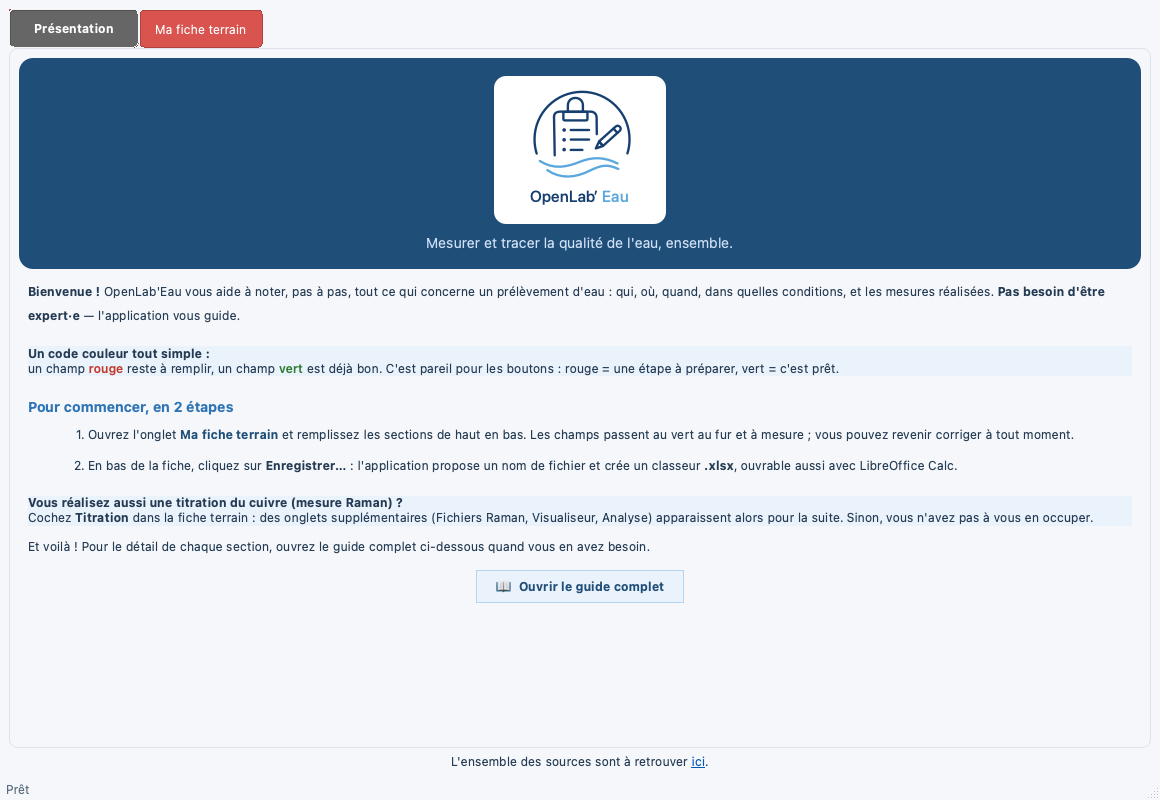
\includegraphics[width=0.74\linewidth]{captures_openlabeau/ov_fenetre.png}}}\\[4pt]
  {\small\color{darkgray} Vue générale d'OpenLab'Eau, fenêtre ouverte.}

  \vfill

  {\color{darkgray}\small
    \textbf{CitizenSers} : document à usage interne.\\[6pt]
    Pour toute question, contactez la personne responsable
    du prélèvement.
  }
\end{titlepage}

\newpage
\tableofcontents
\newpage

% ══════════════════════════════════════════════════════════════
\section{Avant de commencer}
% ══════════════════════════════════════════════════════════════

\subsection{À quoi sert OpenLab'Eau}

OpenLab'Eau vous aide à noter tout ce qui concerne un prélèvement d'eau.
Qui a prélevé, où, quand, dans quelles conditions, et quelles mesures ont
été faites.

Vous remplissez une \textbf{fiche terrain}. Le logiciel l'enregistre dans
un fichier Excel propre et bien rangé. C'est ce fichier que l'on garde et
que l'on partage.

Si vous faites aussi une \textbf{titration du cuivre} (la mesure au laser
Raman), OpenLab'Eau vous accompagne en plus pour préparer les tubes,
regarder les spectres et trouver le résultat. Cette partie est expliquée
plus loin. Si vous ne faites pas de titration, vous pouvez l'ignorer.

\begin{conseil}
  Pas besoin de comprendre la physique du laser pour utiliser le logiciel.
  Il suffit de remplir les cases dans l'ordre. Le logiciel fait le reste.
\end{conseil}

\subsection{Le code couleur, tout simple}

OpenLab'Eau utilise deux couleurs partout.

\begin{itemize}
  \item Un champ \rouge{rouge} reste à remplir.
  \item Un champ \vertok{vert} est déjà bon.
\end{itemize}

C'est pareil pour les boutons. Un bouton rouge veut dire une étape à
préparer. Un bouton vert veut dire que c'est prêt. Vous savez donc
toujours ce qu'il reste à faire d'un coup d'œil.

\subsection{Les onglets}

Les onglets sont les boutons en haut de la fenêtre. Au départ, vous en
voyez deux.

\begin{itemize}
  \item \onglet{Présentation} : un petit accueil et un bouton vers le
        guide complet. Rien à remplir ici.
  \item \onglet{Ma fiche terrain} : c'est là que vous travaillez. Vous
        remplissez les sections du haut vers le bas.
\end{itemize}

Trois autres onglets apparaissent \textbf{seulement} si vous cochez
\champ{Titration du cuivre} dans la fiche terrain.

\begin{itemize}
  \item \onglet{Fichiers Raman} : vous choisissez les fichiers de spectres
        et vous dites quel spectre va avec quel tube.
  \item \onglet{Visualiseur} : vous regardez les spectres tracés.
  \item \onglet{Analyse} : le logiciel suit les pics et trouve le
        résultat.
\end{itemize}

\begin{enresume}
  Sans titration, vous n'avez besoin que de l'onglet
  \onglet{Ma fiche terrain}. Avec titration, trois onglets en plus
  apparaissent pour la suite.
\end{enresume}

\begin{figure}[H]
  \centering
  {\setlength{\fboxsep}{0pt}\setlength{\fboxrule}{0.5pt}%
   \fbox{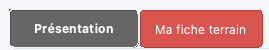
\includegraphics[width=0.42\linewidth]{captures_openlabeau/onglets_base.png}}}\\[8pt]
  {\setlength{\fboxsep}{0pt}\setlength{\fboxrule}{0.5pt}%
   \fbox{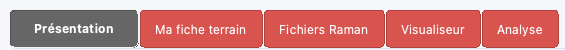
\includegraphics[width=0.80\linewidth]{captures_openlabeau/onglets_titration.png}}}
  \caption{En haut, les deux onglets de départ. En bas, les cinq onglets
           une fois la titration cochée.}
\end{figure}

\newpage

% ══════════════════════════════════════════════════════════════
\section{Remplir ma fiche terrain}
% ══════════════════════════════════════════════════════════════

\subsection{Ouvrir ou reprendre une fiche}

Cliquez sur l'onglet \onglet{Ma fiche terrain}.

Pour repartir d'une fiche vide, le bouton \bouton{Nouvelle fiche} est en
haut. Pour reprendre une fiche déjà commencée, cliquez sur
\bouton{Charger une fiche\ldots} en haut, puis choisissez votre fichier
Excel.

Sinon, remplissez simplement les sections de haut en bas. Les champs
passent au vert au fur et à mesure. Vous pouvez revenir corriger à tout
moment.

\figcap[0.9\linewidth]{fiche_terrain.png}{%
  La fiche terrain en cours de remplissage. Les champs verts sont bons, les
  champs rouges restent à faire. Le nom du prélèvement se crée tout seul.}

\subsection{Le prélèvement}

Cette section dit qui a prélevé, où et quand.

\etape{1}{Les personnes qui ont prélevé}

Écrivez chaque personne au format \textbf{prénom puis nom}, avec son
association sur la même ligne. Pour ajouter quelqu'un, cliquez sur
\bouton{+1 préleveur·se}.

\etape{2}{La date et l'heure}

Renseignez la date et l'heure du prélèvement. Elles sont vides au départ
et passent au vert une fois remplies.

\etape{3}{Le lieu}

Entrez la latitude et la longitude. Vous pouvez taper des coordonnées GPS
ou utiliser le bouton \bouton{Carte / pointer\ldots} pour placer le point
sur une carte. Si vous avez Internet, le département et la commune se
remplissent tout seuls. Vous pouvez quand même les corriger à la main.

\begin{conseil}
  Le \textbf{nom du prélèvement} se crée tout seul dès que les initiales
  et la date sont là. Il ressemble à \texttt{PRE\_DJAM\_20260430\_14h00}.
  Ce nom est comme le code-barres de votre sortie. Vérifiez qu'il est
  unique avant d'enregistrer.
\end{conseil}

\subsection{Le contexte}

Cette section décrit l'eau et la météo au moment du prélèvement.

\etape{4}{Le type d'eau}

Choisissez \champ{Eau douce}, \champ{Eau de mer} ou
\champ{Eau estuarienne}. Tant que rien n'est choisi, la case reste rouge.

Selon votre choix, des champs en plus apparaissent. Pour l'eau de mer ou
estuarienne, le logiciel demande le coefficient de marée et l'heure de
pleine mer. Pour l'eau douce, il demande le débit du cours d'eau.

\etape{5}{Les conditions}

Remplissez la température de l'eau, la météo, la température de l'air, la
pluie des dernières 24 heures et un commentaire libre. Ces infos aident à
comprendre le prélèvement plus tard.

\subsection{Les mesures faites}

Cochez les mesures que vous avez réalisées. Chaque case ouvre les champs
qui vont avec.

\begin{itemize}
  \item \champ{Test ammonium} : ouvre les champs du test, le pH et la
        personne qui l'a fait.
  \item \champ{Turbidité mesurée} : pour noter la turbidité.
  \item \champ{Conductivité mesurée} : pour noter la conductivité.
  \item \champ{pH de l'eau mesuré} : pour noter le pH.
  \item \champ{Oxygène dissous mesuré} : pour noter l'oxygène dissous.
  \item \champ{Analyses bactériologiques} : pour le jour et l'heure de
        dépôt, le laboratoire et les résultats E. coli et entérocoques
        s'ils sont déjà connus.
  \item \champ{Titration du cuivre} : à cocher seulement si vous faites
        la mesure au Raman. Elle ouvre toute la partie titration, décrite
        à la section suivante.
\end{itemize}

\begin{attention}
  Ne cochez que les mesures que vous avez vraiment faites. Une case cochée
  mais laissée vide donnera juste un petit avertissement à
  l'enregistrement.
\end{attention}

\subsection{Enregistrer la fiche}

\etape{6}{Enregistrer}

Cliquez sur \bouton{Enregistrer la fiche\ldots} tout en bas. Le logiciel
propose un nom de fichier basé sur votre prélèvement. Cliquez sur
\bouton{Enregistrer}.

Le fichier est un classeur Excel (\texttt{.xlsx}). LibreOffice Calc peut
aussi l'ouvrir et le réenregistrer.

Le nom du fichier ajoute de petites étiquettes selon ce que vous avez
coché. Par exemple \texttt{\_T} pour la titration, \texttt{\_AnBa} pour les
analyses bactériologiques, \texttt{\_pH} pour le pH, et ainsi de suite.
Vous repérez donc le contenu d'un fichier rien qu'à son nom.

\begin{conseil}
  Enregistrez régulièrement. Si vous fermez le logiciel sans enregistrer,
  ce que vous avez tapé est perdu.
\end{conseil}

\begin{enresume}
  Si vous ne faites pas de titration, c'est terminé. Votre fiche terrain
  est enregistrée et prête à être partagée. La suite ne concerne que la
  titration du cuivre.
\end{enresume}

\newpage

% ══════════════════════════════════════════════════════════════
\section{La titration du cuivre (mesure Raman)}
% ══════════════════════════════════════════════════════════════

\subsection{L'idée, en deux mots}

On veut connaître la quantité de cuivre dans l'eau. Pour cela, on ajoute
petit à petit une solution dont on connaît la concentration. C'est la
\textbf{titration}.

À un moment précis, il y a juste ce qu'il faut de solution ajoutée pour
réagir avec tout le cuivre. C'est le \textbf{point d'équivalence}. Le
laser Raman nous donne une signature lumineuse de chaque tube. En suivant
comment cette signature change, on repère ce point. On en déduit la
quantité de cuivre du départ.

OpenLab'Eau vous accompagne pour préparer les tubes, regarder les spectres
et trouver ce point d'équivalence.

\begin{conseil}
  Pas besoin de comprendre tout le détail. L'important est l'idée : on
  ajoute du titrant tube après tube, et on regarde à partir de quel moment
  ça change nettement.
\end{conseil}

\subsection{Cocher la titration}

Dans \onglet{Ma fiche terrain}, cochez \champ{Titration du cuivre}. Une
section titration s'ouvre, et trois onglets apparaissent en haut :
Fichiers Raman, Visualiseur et Analyse.

Dans la section titration, renseignez le coordinateur·ice et
l'opérateur·ice au format prénom puis nom, puis le lieu, la date et
l'heure. Le \textbf{nom de la manip} se crée tout seul. Le bouton
\bouton{Modifier} permet d'entrer un nom à la main si besoin.

\subsection{Préparer les tubes}

\etape{1}{Choisir le modèle de volumes}

Le tableau des volumes dit combien de chaque solution mettre dans chaque
tube. Choisissez le modèle proposé, puis cliquez sur
\bouton{Valider le modèle}. Pour un usage avancé, le bouton
\bouton{Générer un tableau de volume\ldots} permet de tout régler à la
main.

\etape{2}{Sortir la feuille de protocole}

Cliquez sur \bouton{Feuille de protocole\ldots}. Vous pouvez la remplir
directement dans le logiciel, ou l'imprimer pour la remplir à la main à la
paillasse. Elle donne, pour chaque tube, le volume exact de chaque
solution, avec des cases à cocher.

\figph[La feuille de protocole.]{%
  Capture de la feuille de protocole : un tube par colonne,
  une solution par ligne, des cases à cocher au fur et à mesure.}

\begin{conseil}
  Cette feuille est très pratique à deux. Une personne annonce les
  volumes, l'autre pipette et coche. Les cases servent de garde-fou pour
  éviter les erreurs.
\end{conseil}

\subsection{Étape : Fichiers Raman}

Une fois les spectres acquis avec le spectromètre, ouvrez l'onglet
\onglet{Fichiers Raman}.

\etape{3}{Choisir les fichiers}

Cliquez sur \bouton{Choisir des fichiers Raman (.txt)\ldots}. La fenêtre
de votre ordinateur s'ouvre. Choisissez tous les fichiers de votre manip
d'un coup, puis validez. Ils s'affichent dans la liste
\champ{Fichiers sélectionnés}.

Pour enlever un fichier ajouté par erreur, cliquez dessus puis sur
\bouton{Retirer la sélection}. Pour tout enlever, cliquez sur
\bouton{Vider la liste}.

\begin{attention}
  Ne prenez que les fichiers \texttt{.txt} de cette manip. Mélanger les
  fichiers d'une autre expérience fausserait le résultat.
\end{attention}

\figcap[0.92\linewidth]{fichiers_raman.png}{%
  L'onglet Fichiers Raman : le bouton bleu pour choisir les fichiers, la liste
  des spectres retenus, et en dessous l'étape pour les associer aux tubes.}

\etape{4}{Associer les spectres aux tubes}

Juste en dessous, une zone \champ{Étape suivante --- associer les spectres
aux tubes} vous attend. Cliquez sur son bouton pour ouvrir le tableau de
correspondance. Là, vous dites quel fichier spectre va avec quel tube.

Le petit voyant passe au vert quand tout est associé. L'onglet
\onglet{Fichiers Raman} devient vert lui aussi quand les fichiers sont
choisis et la correspondance prête.

\begin{attention}
  Si vous avez fait deux spectres pour le même tube, donnez le même numéro
  de tube aux deux fichiers.
\end{attention}

\subsection{Étape : Visualiseur}

Ouvrez l'onglet \onglet{Visualiseur} pour regarder vos spectres et
vérifier qu'ils sont propres.

\etape{5}{Tracer les spectres}

Cliquez sur \bouton{Tracer les spectres}. Chaque courbe est un spectre.
Le nom du fichier sert de légende. Cochez ou décochez un spectre pour
l'afficher ou le cacher.

Le graphique est interactif. Vous pouvez zoomer en dessinant un rectangle
avec la souris, vous déplacer, et revenir à la vue complète en
double-cliquant. Les champs \champ{X min}, \champ{X max}, \champ{Y min} et
\champ{Y max} avec le bouton \bouton{Appliquer les axes} permettent de
cadrer la vue. Le bouton \bouton{Y auto} remet la hauteur automatiquement.

\figcap{visualiseur.png}{%
  L'onglet Visualiseur : les spectres tracés et colorés, avec la légende
  par nom de fichier sur le côté.}

\begin{conseil}
  Si un spectre a l'air bizarre (très bruité, pic qui manque), notez son
  nom. Vérifiez la correspondance spectres et tubes avant de passer à
  l'analyse.
\end{conseil}

\subsection{Étape : Analyse}

Ouvrez l'onglet \onglet{Analyse}. Le logiciel suit la hauteur des pics en
fonction de la quantité de titrant ajoutée. Il lit tout seul la quantité
de titrant de chaque tube grâce à la fiche terrain.

\etape{6}{Détecter les pics}

Réglez si besoin la fenêtre dans la section \champ{Fenêtre \& détection}.
La case \champ{Corriger la ligne de base} est là pour nettoyer le fond du
signal. Cliquez ensuite sur \bouton{1) Détecter les pics}.

\etape{7}{Choisir les pics à suivre}

Les pics trouvés s'affichent dans \champ{Pics détectés}. Cochez ceux que
vous voulez suivre. Les boutons \bouton{Tout cocher} et
\bouton{Tout décocher} font gagner du temps.

\etape{8}{Tracer la hauteur des pics}

Cliquez sur \bouton{2) Tracer la hauteur des pics}. Le graphique montre,
pour chaque pic coché, comment sa hauteur évolue quand on ajoute du
titrant.

\figcap{analyse.png}{%
  L'onglet Analyse : la hauteur des pics suivie en fonction de la quantité de
  titrant. La courbe en pointillés marque le point d'équivalence.}

\etape{9}{Trouver l'équivalence}

Cochez la case dans la zone \champ{Équivalence (fin de la droite)}. Le
logiciel ajuste une courbe en forme de S sur les points. Le point
d'équivalence est l'endroit où la montée se termine. C'est lui qui donne
la quantité de cuivre.

\begin{attention}
  Si la courbe ne colle pas du tout aux points mesurés, c'est souvent que
  ce pic n'est pas le bon à suivre. Essayez un autre pic. Si ça ne va
  toujours pas, demandez à la personne responsable.
\end{attention}

\etape{10}{Exporter les résultats}

Vous pouvez tout enregistrer. Cliquez sur
\bouton{Exporter les résultats (CSV)\ldots} pour un fichier texte simple,
ou sur \bouton{Exporter les résultats (XLSX)\ldots} pour un classeur
Excel. Choisissez l'endroit et le nom, puis enregistrez.

\begin{enresume}
  À la fin, vous avez vos spectres vérifiés, la hauteur des pics suivie, le
  point d'équivalence, et un fichier de résultats. La titration est
  terminée.
\end{enresume}

\newpage

% ══════════════════════════════════════════════════════════════
\section{Le parcours en un coup d'œil}
% ══════════════════════════════════════════════════════════════

\begin{center}
\begin{tikzpicture}[node distance=0.45cm]

  \tikzstyle{stepbox} = [
    rounded corners=5pt,
    draw=none,
    minimum width=11cm, minimum height=1.0cm,
    align=left, text width=10.3cm,
    font=\small, text=white
  ]

  \node[stepbox, fill=tab5col] (s1)
    {{\bfseries 1.}\enskip
     Ouvrir l'onglet \textbf{Ma fiche terrain}};

  \node[stepbox, fill=tab5col!90!wflight, below=of s1] (s2)
    {{\bfseries 2.}\enskip
     Remplir le prélèvement, le contexte et les mesures faites};

  \node[stepbox, fill=tab5col!80!wflight, below=of s2] (s3)
    {{\bfseries 3.}\enskip
     Enregistrer la fiche en \texttt{.xlsx}\quad (fin si pas de titration)};

  \node[stepbox, fill=tab5col!66!wflight, below=of s3] (s4)
    {{\bfseries 4.}\enskip
     Cocher \textbf{Titration du cuivre}, valider le modèle de volumes};

  \node[stepbox, fill=tab5col!56!wflight, below=of s4] (s5)
    {{\bfseries 5.}\enskip
     Sortir la feuille de protocole pour la paillasse};

  \node[stepbox, fill=tab5col!46!wflight, below=of s5] (s6)
    {{\bfseries 6.}\enskip
     Onglet \textbf{Fichiers Raman} : choisir les \texttt{.txt}};

  \node[stepbox, fill=tab5col!36!wflight, below=of s6] (s7)
    {{\bfseries 7.}\enskip
     Associer chaque spectre à son tube};

  \node[stepbox, fill=tab5col!26!wflight, below=of s7] (s8)
    {{\bfseries 8.}\enskip
     Onglet \textbf{Visualiseur} : tracer et vérifier les spectres};

  \node[stepbox, fill=tab5col!16!wflight, below=of s8] (s9)
    {{\bfseries 9.}\enskip
     Onglet \textbf{Analyse} : détecter les pics, choisir ceux à suivre};

  \node[stepbox, fill=wflight, below=of s9] (s10)
    {{\bfseries 10.}\enskip
     Tracer la hauteur, lire l'équivalence, exporter les résultats};

  \draw[->, thick, color=tab5col!60!white] (s1.south) -- (s2.north);
  \draw[->, thick, color=tab5col!60!white] (s2.south) -- (s3.north);
  \draw[->, thick, color=tab5col!60!white] (s3.south) -- (s4.north);
  \draw[->, thick, color=tab5col!60!white] (s4.south) -- (s5.north);
  \draw[->, thick, color=tab5col!60!white] (s5.south) -- (s6.north);
  \draw[->, thick, color=tab5col!60!white] (s6.south) -- (s7.north);
  \draw[->, thick, color=tab5col!60!white] (s7.south) -- (s8.north);
  \draw[->, thick, color=tab5col!60!white] (s8.south) -- (s9.north);
  \draw[->, thick, color=tab5col!60!white] (s9.south) -- (s10.north);

\end{tikzpicture}
\end{center}

\newpage

% ══════════════════════════════════════════════════════════════
\section{Reprendre une fiche commencée}
% ══════════════════════════════════════════════════════════════

Si vous avez fermé le logiciel, vous pouvez reprendre là où vous en étiez.

\begin{enumerate}
  \item Ouvrez OpenLab'Eau.
  \item Cliquez sur l'onglet \onglet{Ma fiche terrain}.
  \item Cliquez sur \bouton{Charger une fiche\ldots} en haut.
  \item Choisissez votre fichier \texttt{.xlsx} et ouvrez-le.
  \item Si vous faites une titration, retournez dans
        \onglet{Fichiers Raman} et choisissez à nouveau vos fichiers
        \texttt{.txt}.
  \item Reprenez à l'étape où vous vous étiez arrêté·e.
\end{enumerate}

\begin{conseil}
  Enregistrez souvent. Comme ça, vous ne perdez jamais votre travail, même
  si le logiciel se ferme par accident.
\end{conseil}

% ══════════════════════════════════════════════════════════════
\section{Questions fréquentes}
% ══════════════════════════════════════════════════════════════

\textbf{Je ne vois pas les onglets Fichiers Raman, Visualiseur et Analyse.}

C'est normal s'il n'y a pas de titration. Cochez
\champ{Titration du cuivre} dans la fiche terrain et ils apparaissent.

\bigskip

\textbf{Un champ reste rouge alors que j'ai écrit dedans.}

Vérifiez qu'il n'est pas vide et que le format est bon (une date dans un
champ date, par exemple). Le rouge veut juste dire qu'il manque encore
quelque chose.

\bigskip

\textbf{Le graphique des spectres est vide.}

Vérifiez d'abord que des fichiers sont bien choisis dans l'onglet
\onglet{Fichiers Raman}. Puis revenez au \onglet{Visualiseur} et cliquez
sur \bouton{Tracer les spectres}.

\bigskip

\textbf{La courbe d'équivalence ne colle pas aux points.}

Le pic suivi n'est sans doute pas le bon. Choisissez un autre pic dans la
liste des pics détectés et tracez à nouveau. Si ça ne va toujours pas,
demandez à la personne responsable.

\bigskip

\textbf{Puis-je enregistrer sans avoir tout rempli ?}

Oui. Vous pouvez enregistrer même incomplet. Le logiciel signale juste les
points à vérifier, sans bloquer.

\bigskip

\textbf{Puis-je ouvrir le fichier sans OpenLab'Eau ?}

Oui. C'est un fichier Excel. Vous l'ouvrez avec Excel ou avec LibreOffice
Calc.

% ──────────────────────────────────────────────────────────────
\vfill
\begin{center}
  \color{rulecolor}\rule{8cm}{0.4pt}\\[6pt]
  \small\color{darkgray}
  Document rédigé pour CitizenSers.\\
  Pour toute question, contactez la personne responsable du prélèvement.
\end{center}

\end{document}
